\documentclass{commsummary}

% 可以在这里添加额外的宏包或定义(pgfplots 已移至 cls 文件中)

\title{\textbf{\huge 通信原理核心公式速查}}
\author{复习笔记}
\date{\today}

\raggedbottom

\begin{document}

\maketitle

% 插入目录(可选,如果你想概览)
% \tableofcontents
% \newpage

% --- 导入各章内容 ---
% 注意:你的 tex 文件都在 chapter 文件夹下,所以路径要是 chapter/文件名

\section{绪论与信号基础} 
    \section{绪论与信号基础}

% --- 模块一:傅里叶变换 (核心理论) ---
\begin{kbox}{信号分析基础:傅里叶变换}
    \begin{enumerate}
        \item \textbf{定义} \pptpage{6}
        \begin{itemize}
            \item 正变换:$F(\omega)=\int_{-\infty}^{\infty} f(t) e^{-j \omega t} d t$
            \item 反变换:$f(t)=\frac{1}{2 \pi} \int_{-\infty}^{\infty} F(\omega) e^{j \omega t} d \omega$
        \end{itemize}

        \item \textbf{常用运算特性} \pptpage{7-8}
        \begin{itemize}
            \item \textbf{共轭对称性}(补充):
            实信号 $f(t)$ 的频谱满足 $F(\omega) = F^*(-\omega)$。
            即:\textbf{幅度谱为偶函数,相位谱为奇函数}。
            \item \textbf{标度换算}:
            $f(a t) \leftrightarrow \frac{1}{|a|} F\left(\frac{\omega}{a}\right)$
            \item \textbf{时移特性}:
            $f(t-t_{0}) \leftrightarrow e^{-j \omega t_{0}} F(\omega)$
            \item \textbf{频移特性}:
            $e^{j \omega_{0} t} f(t) \leftrightarrow F(\omega-\omega_{0})$
            \item \textbf{调制特性}:
            $f(t) \cos \omega_{0} t \leftrightarrow \frac{1}{2}[F(\omega+\omega_{0})+F(\omega-\omega_{0})]$
            \item \textbf{时域卷积}:
            $f_{1}(t) * f_{2}(t) \leftrightarrow F_{1}(\omega) \cdot F_{2}(\omega)$
            \item \textbf{微分特性}:
            $\frac{d^{n}}{d t^{n}} f(t) \leftrightarrow(j \omega)^{n} F(\omega)$
        \end{itemize}

        \item \textbf{常用信号对与推论} \pptpage{10-11}
        \begin{itemize}
            \item \textbf{矩形脉冲}(重要):
            宽度为 $\tau$ 的门函数 $g_\tau(t) \leftrightarrow \tau \operatorname{Sa}\left(\frac{\omega \tau}{2}\right)$
            \begin{itemize}
                \item[$\circ$] 注:$Sa(x)=\frac{\sin x}{x}$, $sinc(x)=\frac{\sin \pi x}{\pi x}$
                \item[$\circ$] 关系:$Sa(\frac{\omega\tau}{2}) = sinc(f\tau)$
                \item[$\circ$] \textbf{对偶特性(笔记补充)}:
                $Sa(\tau t) \leftrightarrow \frac{\pi}{\tau} g_{2\tau}(\omega)$
                \\ (含义:时域 Sa 函数对应频域宽度为 $2\tau$ 的矩形谱)
            \end{itemize}
            \item \textbf{三角脉冲}:
            等腰三角脉冲可分解为两个矩形脉冲的卷积。
            
            % --- TikZ 绘图 ---
            \begin{center}
            \begin{tikzpicture}[scale=0.55, >=latex, font=\scriptsize]
                \tikzstyle{axis}=[->, thin, gray]
                \tikzstyle{signal}=[thick, mainblue] 

                % --- 图1:三角波 ---
                \draw[axis] (-1.8,0) -- (1.8,0);
                \draw[axis] (0,-0.2) -- (0,1.8);
                \draw[signal] (-1.2, 0) -- (0, 1.4) node[right, black]{$A^2\tau$} -- (1.2, 0);
                \node[below] at (-1.2, 0) {$-\tau$};
                \node[below] at (1.2, 0) {$\tau$};

                % --- 等号 ---
                \node at (2.2, 0.7) {\large $=$};
                % --- 图2:矩形波1 ---
                \begin{scope}[shift={(4.5,0)}]
                    \draw[axis] (-1.2,0) -- (1.2,0);
                    \draw[axis] (0,-0.2) -- (0,1.8);
                    \draw[signal] (-0.6, 0) -- (-0.6, 1) -- (0.6, 1) node[midway, above, black, xshift=7pt]{$A$} -- (0.6, 0);
                    \node[below] at (-0.6, 0) {$-\frac{\tau}{2}$};
                    \node[below] at (0.6, 0) {$\frac{\tau}{2}$};
                \end{scope}

                % --- 卷积符号 ---
                \node at (6.2, 0.7) {\large $*$};
                % --- 图3:矩形波2 ---
                \begin{scope}[shift={(8,0)}]
                    \draw[axis] (-1.2,0) -- (1.2,0);
                    \draw[axis] (0,-0.2) -- (0,1.8);
                    \draw[signal] (-0.6, 0) -- (-0.6, 1) -- (0.6, 1) node[midway, above, black, xshift=7pt]{$A$} -- (0.6, 0);
                    \node[below] at (-0.6, 0) {$-\frac{\tau}{2}$};
                    \node[below] at (0.6, 0) {$\frac{\tau}{2}$};
                \end{scope}
            \end{tikzpicture}
            \end{center}

            \item \textbf{双边指数信号}:
            $f(t) = e^{-\alpha t}u(t) - e^{\alpha t}u(-t) \leftrightarrow \frac{-2j\omega}{\alpha^2+\omega^2} \quad (\alpha>0)$
            \item \textbf{符号函数}:
            由上式令 $\alpha \to 0$ 可得:$\operatorname{sgn}(t) \leftrightarrow \frac{2}{j\omega}$
            \item \textbf{单位冲激串}:
            $\delta_{T}(t) \leftrightarrow \omega_{0} \sum_{n=-\infty}^{\infty} \delta(\omega-n \omega_{0})$
        \end{itemize}
    \end{enumerate}
\end{kbox}      % 核心公式
    % --- 模块一补充:笔记推导细节 ---
\begin{examplebox}{笔记补充:Sa函数与门函数的对偶性推导}
    \textbf{1. 基础变换回顾}
    \begin{itemize}
        \item 门函数 $\to$ Sa函数:
        \[ g_{\tau}(t) \longleftrightarrow \tau Sa\left(\frac{\omega \tau}{2}\right) \]
        \item Sa函数 $\to$ 门函数(利用对偶性):
        \[ Sa(\Omega t) \longleftrightarrow \frac{\pi}{\Omega} g_{2\Omega}(\omega) \]
    \end{itemize}
    
    \tcbline % 分割线
    
    \textbf{2. 频域 $f$ 下的对应关系推导}
    
    \textit{问题:如何将 $Sa(\Omega t)$ 的频谱表示为关于 $f$ 的门函数?}
    
    \begin{itemize}
        \item \textbf{变量代换}:
        已知角频率与频率关系为 $w = 2\pi f$。
        \item \textbf{带宽边界映射}:
        对于频域门函数 $g_{2\Omega}(\omega)$,其截止角频率为 $w = \pm \Omega$(宽度为 $2\Omega$)。
        \item \textbf{计算 $f$ 域宽度}:
        当 $w = \Omega$ 时,对应的频率 $f$ 为:
        \[ f = \frac{w}{2\pi} = \frac{\Omega}{2\pi} \]
        因此,总宽度(即门函数的下标)为:
        \[ \text{Width}_f = \frac{\Omega}{2\pi} - \left(-\frac{\Omega}{2\pi}\right) = \frac{\Omega}{\pi} \]
        \item \textbf{最终结论}:
        \[ \frac{\Omega}{\pi} Sa(\Omega t) \longleftrightarrow g_{\frac{\Omega}{\pi}}(f) \]
    \end{itemize}
\end{examplebox} % <--- 【新增】笔记补充推导
    % --- 模块:常用变换速查表 ---
\begin{kbox}{速查表:常用函数傅里叶变换对}
    \begin{center}
    \renewcommand{\arraystretch}{1.5}
    \begin{tabular}{c|c}
        \hline
        \textbf{时域信号} $f(t)$ & \textbf{频域频谱} $F(\omega)$ \\
        \hline
        $\delta(t)$ & $1$ \\
        $1$ & $2\pi \delta(\omega)$ \\
        $u(t)$ & $\pi \delta(\omega) + \frac{1}{j\omega}$ \\
        $e^{-\alpha t}u(t) \ (\alpha > 0)$ & $\frac{1}{\alpha + j\omega}$ \\
        $e^{-\alpha |t|} \ (\alpha > 0)$ & $\frac{2\alpha}{\alpha^2 + \omega^2}$ \\
        $e^{j \omega_0 t}$ & $2\pi \delta(\omega - \omega_0)$ \\
        $\cos(\omega_0 t)$ & $\pi [\delta(\omega - \omega_0) + \delta(\omega + \omega_0)]$ \\
        $\sin(\omega_0 t)$ & $j\pi [\delta(\omega + \omega_0) - \delta(\omega - \omega_0)]$ \\
        $\operatorname{sgn}(t)$ & $\frac{2}{j\omega}$ \\
        \hline
    \end{tabular}
    \end{center}
\end{kbox}

% --- 模块:w与f域性质对比 ---
\begin{kbox}{深度对比:$\omega$ 与 $f$ 域性质差异}
    \textbf{核心差异速记}:
    \begin{itemize}
        \item \textbf{积分相关}(逆变换、卷积、能量):$\omega$ 域通常需乘 $\frac{1}{2\pi}$ 修正。
        \item \textbf{微分相关}:$f$ 域通常需乘 $2\pi$。
    \end{itemize}
    
    \begin{center}
    \renewcommand{\arraystretch}{1.3}
    \resizebox{\linewidth}{!}{
    \begin{tabular}{c|c|c}
        \hline
        \textbf{性质} & \textbf{$\omega$ 域 (rad/s)} & \textbf{$f$ 域 (Hz)} \\
        \hline
        \textbf{逆变换} & $\frac{1}{2\pi} \int F(\omega)e^{j\omega t}d\omega$ & $\int F(f)e^{j2\pi ft}df$ \\
        \hline
        \textbf{频域卷积} & $\frac{1}{2\pi} [F_1 * F_2]$ & $F_1 * F_2$ \\
        {\scriptsize (对应时域相乘)} & {\scriptsize (需除系数)} & {\scriptsize (无系数,对称)} \\
        \hline
        \textbf{能量} & $\frac{1}{2\pi} \int |F(\omega)|^2 d\omega$ & $\int |F(f)|^2 df$ \\
        \hline
        \textbf{时域微分} & $(j\omega)^n F(\omega)$ & $(j2\pi f)^n F(f)$ \\
        \hline
        \textbf{直流 DC} & $2\pi\delta(\omega)$ & $\delta(f)$ \\
        \hline
    \end{tabular}
    }
    \end{center}
\end{kbox}
    % --- 模块二:确定信号与系统 ---
\begin{kbox}{确定信号性质与线性系统}
    \begin{enumerate}
        \item \textbf{能量与功率} \pptpage{14}
        \begin{itemize}
            \item 能量:$E=\int_{-\infty}^{\infty} s^{2}(t) d t$
            \item 功率:$P=\lim _{T \rightarrow \infty} \frac{1}{T} \int_{-T / 2}^{T / 2} s^{2}(t) d t$
        \end{itemize}

        \item \textbf{带宽定义} \pptpage{15}
        \begin{equation*}
            B_{3}=\frac{\int_{-\infty}^{\infty} E(f) d f}{2 E(0)} \quad (\text{等效矩形带宽})
        \end{equation*}

        \item \textbf{线性系统响应} \pptpage{16-17}
        \begin{itemize}
            \item 频域:$Y(f)=H(f) X(f)$
            \item 时域:$y(t)=\int_{-\infty}^{\infty} h(t-\tau) x(\tau) d \tau$
        \end{itemize}
        
        \item \textbf{无失真传输条件} \pptpage{18} 
        \begin{itemize}
            \item 时域条件:$y(t)=k x(t-t_{d})$
            \item 频域条件:$H(\omega)=K e^{-j \omega t_{d}}$
            \item \textbf{群时延}:$\tau(\omega)=-\frac{d \varphi(\omega)}{d \omega} = \text{常数}$
        \end{itemize}
    \end{enumerate}
\end{kbox}
    % --- 模块三:信息论基础 ---
\begin{kbox}{信息及其度量}
    \begin{enumerate}
        \item \textbf{离散消息信息量} \pptpage{50}
        \begin{equation*}
            I = -\ln P(x) \quad (\text{单位 nat})
        \end{equation*}
        \textbf{单位换算}:
        \begin{itemize}
            \item $I_{bit} = -\log_2 P(x) = \frac{1}{\ln 2} I_{nat}$
            \item $1 \text{ nat} \approx 1.44 \text{ bit}$
        \end{itemize}

        \item \textbf{离散信源熵 (平均信息量)} \pptpage{52}
        \begin{equation*}
            H=\sum_{i=1}^{M} P(x_{i}) \log _{2} \frac{1}{P(x_{i})} \quad (\text{bit/符号})
        \end{equation*}
        \textbf{最大熵}:当等概率出现时,$H_{\max }=\log _{2} M$。

        \item \textbf{总信息量} \pptpage{55}
        \begin{equation*}
            I_{\text{总}} = m \cdot H \quad (m \text{为符号总数})
        \end{equation*}
    \end{enumerate}
\end{kbox}
    % --- 模块四:信道模型 ---
\begin{kbox}{信道与衰落}
    \begin{enumerate}
        \item \textbf{调制信道模型} \pptpage{59}
        \begin{equation*}
            e_{o}(t)=k(t) e_{i}(t)+n(t)
        \end{equation*}

        \item \textbf{多径效应与正交分解} \pptpage{70}
        接收信号 $R(t)$ 为多径叠加:
        \begin{align*}
            R(t) &= \sum_{i=1}^{n} \mu_i(t) \cos[\omega_c (t - \tau_i(t))] \\
                 & \qquad \text{\small (原始多径公式)} \\
                 &= \sum_{i=1}^{n} \mu_i(t) \cos[\omega_c t + \varphi_i(t)] \\
                 & \quad {\color{red}\text{其中 } \varphi_i(t) = -\omega_c \tau_i(t) } \\ 
                 &= \sum_{i=1}^{n} \mu_i(t) \cos(\omega_c t) \cos(\varphi_i(t)) \\
                 &\quad - \sum_{i=1}^{n} \mu_i(t) \sin(\omega_c t) \sin(\varphi_i(t)) \\
                 &= X_c(t) \cos(\omega_c t) - X_s(t) \sin(\omega_c t) \\
                 &= V(t) \cos[\omega_c t + \varphi(t)]
        \end{align*}
        \textbf{参数含义}:
        \begin{itemize}
            \item $\mu_i(t)$:第 $i$ 条路径接收信号的\textbf{振幅}。
            \item $\tau_i(t)$:第 $i$ 条路径接收信号的\textbf{时延}。
            \item $\varphi_i(t)$:第 $i$ 条路径接收信号的\textbf{相位},且 $\varphi_i(t) = -\omega_c \tau_i(t)$。
            \item $X_c(t), X_s(t)$:同相与正交分量,大量路径叠加时视为高斯随机过程。
            \item $V(t)$:包络,服从瑞利分布;$\varphi(t)$:合成相位,服从均匀分布。
        \end{itemize}

        \item \textbf{衰落类型与相干带宽} \pptpage{74}
        \begin{itemize}
            \item 相干带宽:$\Delta f \approx 1 / \tau_{m}$ ($\tau_{m}$ 为最大多径时延差)
            \item \textbf{平坦衰落}:信号带宽 $B < \Delta f$
            \item \textbf{频率选择性衰落}:信号带宽 $B > \Delta f$
        \end{itemize}
    \end{enumerate}
\end{kbox}
    % --- 模块五:性能指标 ---
\begin{kbox}{通信系统性能指标}
    \begin{enumerate}
        \item \textbf{模拟系统} \pptpage{87}
        \begin{equation*}
            \text{SNR}(\text{dB}) = 10 \lg (S_{i} / N_{i})
        \end{equation*}

        \item \textbf{补充定义:码元}
        \begin{itemize}
            \item 定义:承载信息的基本单位,是通信的“字符”或“信号”。
            \item 形式:固定时长的脉冲或波形(二进制2种,四进制4种)。
        \end{itemize}

        \item \textbf{数字系统:有效性 (速率)} \pptpage{88-89}
        \begin{itemize}
            \item \textbf{码元速率 ($R_B$)}:波特率(Baud),每秒传送的波形数(“货车”数量)。
            \item \textbf{信息速率 ($R_b$)}:比特率(bps),每秒传送的信息总量(“货物”总量)。
            \item \textbf{关系}:$R_{b} = R_{B} \log _{2} M$
                \begin{itemize}
                    \item 仅当各码元等概出现时,单码元信息量 $I = \log_2 M$。
                \end{itemize}
            \item \textbf{频带利用率}:$\eta = \frac{R_{B}}{B}$ (Baud/Hz) 或 $\frac{R_{b}}{B}$ (bps/Hz)。
        \end{itemize}

        \item \textbf{数字系统:可靠性 (误码/误信)} \pptpage{90-91}
        {\raggedright
        \begin{itemize}
            \item \textbf{误码率 ($P_e$)}:错误码元数占比,$P_e = n_{eB} / n_B$。
                \begin{itemize}
                    \item 二进制平均误码率:$P_e = P(0)P(1|0) + P(1)P(0|1)$。
                \end{itemize}
            \item \textbf{误信率 ($P_b$)}:错误比特数占比,$P_b = n_{eb} / n_b$。
            \item \textbf{关系}:
            \begin{itemize}
                \item 二进制 ($M=2$):$P_{b} = P_{e}$
                \item 多进制 ($M>2$):$P_{b} < P_{e}$
            \end{itemize}
        \end{itemize}
        }
    \end{enumerate}
\end{kbox}

\clearpage  % 用于强制换页

\section{随机过程}
    \begin{kbox}{1. 随机过程定义与统计特性}
    \textbf{定义}:
    随时间作随机变化的一系列随机变量的集合。
        \begin{itemize}[leftmargin=3em]
            \item[(1)] 结构上是:所有样本函数 $\xi_i(t)$ 的集合;
            \item[(2)] 也是随机变量 $\xi(t)$ 的集合。
        \end{itemize}

    \tcbline

    \textbf{统计特性与物理意义}:
    \begin{itemize}
        \item \textbf{一维分布函数}:
        \[ F_1(x_1, t_1) = P\{\xi(t_1) \leq x_1\} \]
        \item \textbf{一维概率密度函数 (PDF)}:
        \[ f_1(x_1, t_1) = \frac{\partial F_1(x_1, t_1)}{\partial x_1} \]
        \item \textbf{均值 (数学期望)} —— \textcolor{mainblue}{直流分量}:
        \[ \mu(t) = E[\xi(t)] = \int_{-\infty}^{\infty} x f_1(x, t) dx \]
        \item \textbf{方差} —— \textcolor{mainblue}{交流功率}:
        \[ \sigma^2(t) = D[\xi(t)] = E\left[(\xi(t) - \mu(t))^2\right] \]
        \item \textbf{平均功率 (二阶原点矩)}:
        由 $DX = E(X^2) - (EX)^2$ 可知功率关系:
        \[ \underbrace{E[\xi^2(t)]}_{\text{平均功率}} = \underbrace{\sigma^2(t)}_{\text{交流功率}} + \underbrace{\mu^2(t)}_{\text{直流功率}} \]
        (当 $\mu(t)=0$ 时,平均功率等于交流功率)
        
        \item \textbf{自相关函数}:
        描述同一过程在任意两个时刻随机变量间的关联程度。
        \begin{align*}
            R(t_1, t_2) &= E[\xi(t_1)\xi(t_2)] \\
            &= \iint_{-\infty}^{\infty} x_1 x_2 f_2(x_1, x_2; t_1, t_2) dx_1 dx_2
        \end{align*}
        (其中 $f_2$ 为二维概率密度函数)
        
        \item \textbf{互相关函数}:
        \[ R_{\xi\eta}(t_1, t_2) = E[\xi(t_1)\eta(t_2)] \]
    \end{itemize}
\end{kbox}

% --- 核心概念辨析 ---
\begin{kbox}{核心概念辨析:样本函数 vs 随机变量}
    \textbf{误区}:随机过程的“样本”不是随机变量,二者观察维度不同。
    
    对于随机过程 $\xi(t, \omega)$:
    \begin{itemize}
        \item \textbf{样本函数 (Sample Function)}:\textcolor{alertred}{固定 $\omega$,变化 $t$}。
        \\ 指随机过程的\textbf{一次具体实现}(如做了一次实验记录下的波形)。既然实验已发生,它就是一条\textbf{确定的时间函数} $x(t)$,不再具有随机性。
        \item \textbf{随机变量 (Random Variable)}:\textcolor{alertred}{固定 $t$,变化 $\omega$}。
        \\ 指随机过程在\textbf{某一特定时刻}的状态。它包含该时刻所有可能的取值及其概率分布,是\textbf{随机的}。
        \item \textbf{总结}:样本函数是“时间的函数”,随机变量是“概率的函数”。二者同时固定时,唯一确定一个数值。
    \end{itemize}
    
    \tcbline
    
    \textbf{直观总结}:
    \begin{itemize}
        \item “样本”是\textbf{纵向的历史轨迹}(确定的曲线)。
        \item “随机变量”是\textbf{横向的时间切片}(统计分布)。
    \end{itemize}
\end{kbox}
    \begin{kbox}{2. 平稳随机过程}
    \textbf{广义平稳 (WSS) 条件}:
    \begin{enumerate}
        \item 均值与时间无关:$\mu(t) = \mu$
        \item 自相关仅与间隔 $\tau$ 有关:$R(t_1, t_1 + \tau) = R(\tau)$
    \end{enumerate}

    \tcbline

    \textbf{狭义平稳 (SSS) 与 广义平稳 (WSS) 对比}:
    \begin{itemize}
        \item \textbf{定义区别}:SSS 要求所有统计特性不变;WSS 仅要求均值和自相关不变。
        \item \textbf{关系}:SSS (二阶矩有限) $\Rightarrow$ WSS;反之通常不成立
        \item \textbf{特例}:对于\textbf{高斯随机过程},WSS $\Leftrightarrow$ SSS。
    \end{itemize}
    
    \tcbline 
    
    \textbf{各态历经性 (遍历性)}:
    \begin{itemize}
        \item \textbf{定义}:若平稳过程的\textbf{统计平均}等于样本的\textbf{时间平均},则称其具有各态历经性。
        \item \textbf{意义}:\textbf{用一次实现的时间平均取代过程的统计平均}。简化测量,因为实际往往只有一个样本波形。
        \item \textbf{数学条件}:$\mu = \bar{\mu}$ 且 $R(\tau) = \bar{R}(\tau)$。
    \end{itemize}
    
    \tcbline
    
    \textbf{深入理解:各态历经性与平稳性的关系}
    \begin{itemize}
        \item \textbf{为什么任一样本能代表整体?} \\
        各态历经的物理含义是:\textbf{一个样本在无限长的时间内,遍历了随机过程所有可能的状态}。因此,观测这一个样本足够久,就等同于观测了整个集合。
        
        \item \textbf{为什么“各态历经 $\Rightarrow$ 平稳”?} \\
        因为“时间平均”是一个常数(积分区间是无穷大),若它等于“统计平均”,则统计平均也必须是常数(不随 $t$ 变化),这正是平稳过程的定义。
        
        \item \textbf{为什么“平稳 $\nRightarrow$ 各态历经”?} \\
        平稳只要求整体统计特性不变,但允许样本之间存在永久性差异(“老死不相往来”)。
        \\ \textit{反例}:$X(t)=C$($C$为随机常数)。样本要么恒为1,要么恒为-1。单个样本的时间平均(1或-1)不等于整体统计平均(0),它没有遍历所有状态。
    \end{itemize}
\end{kbox}
    \begin{kbox}{3. 自相关函数与功率谱密度}
    \textbf{自相关函数 $R(\tau)= E[\xi(t)\xi(t+\tau)]$ 的性质}:
    \begin{enumerate}
        \item 偶函数:$R(\tau) = R(-\tau)$
        \item 最大值:$|R(\tau)| \leq R(0)$
        \item 平均功率:$R(0) = E[\xi^2(t)]$
        \item 直流功率:$R(\infty) = E^2[\xi(t)] = \mu^2$
        \item 交流功率 (方差):$\sigma^2 = R(0) - R(\infty)$
    \end{enumerate}
    
    \vspace{4pt}
    \noindent\tikz\draw[dashed, mainblue!50] (0,0) -- (\linewidth,0);
    \vspace{4pt}
    
    \textbf{\small \textcolor{gray}{性质证明简述 (Proof Sketch)}}
    \small
    \begin{itemize}
        \item \textbf{偶函数}:令 $t' = t-\tau$ 换元,则 $E[\xi(t)\xi(t-\tau)] \Rightarrow E[\xi(t'+\tau)\xi(t')] = R(\tau)$。
        \item \textbf{最大值}:由柯西-施瓦茨不等式 $|E[XY]|^2 \leq E[X^2]E[Y^2]$,令 $X=\xi(t), Y=\xi(t+\tau)$,因平稳性 $E[X^2]=E[Y^2]=R(0)$,得证。
        \item \textbf{直流功率}:当 $\tau \to \infty$,$\xi(t)$ 与 $\xi(t+\tau)$ 去相关 (独立),期望可拆分:$E[\xi(t)\xi(t+\tau)] \approx E[\xi(t)]E[\xi(t+\tau)] = \mu^2$。
        \item \textbf{交流功率}:由方差定义 $\sigma^2 = E[\xi^2] - (E[\xi])^2$,代入即得 $R(0) - R(\infty)$。
    \end{itemize}
    \normalsize
    
    \tcbline
    
    \textbf{维纳-辛钦定理 (PSD)}:
    平稳过程的功率谱密度 $P_{\xi}(\omega)$ 与 $R(\tau)$ 互为傅里叶变换对:
    \begin{align*}
        P_{\xi}(\omega) &= \int_{-\infty}^{\infty} R(\tau) e^{-j\omega\tau} d\tau \\
        R(\tau) &= \int_{-\infty}^{\infty}  P_{\xi}(f) e^{j2\pi f \tau} df
    \end{align*}
\end{kbox}

\begin{kbox}{核心概念辨析:自相关函数值的物理意义}
    \textbf{1. 为什么 $R(0)$ 是总平均功率?}
    \begin{itemize}
        \item \textbf{数学定义}:$R(0) = E[X(t)X(t)] = E[X^2(t)]$,即均方值。
        \item \textbf{物理直观}:$\tau=0$ 时,信号与其自身完全重合,\textbf{相关性最强}。此时记录的是信号在任一时刻的总能量,包含了\textbf{恒定的直流分量}和\textbf{起伏的交流分量}。
    \end{itemize}

    \tcbline

    \textbf{2. 为什么 $R(\infty)$ 是直流功率?}
    \begin{itemize}
        \item \textbf{去相关性 (Decorrelation)}:
        对于非周期的平稳过程,随着时间间隔 $\tau$ 的增大,随机起伏(交流)部分的信号会逐渐失去联系(失去“记忆”)。
        \item \textbf{数学推导}:
        当 $\tau \to \infty$ 时,$X(t)$ 与 $X(t+\tau)$ 变得\textbf{互不相关}。
        \[ \lim_{\tau \to \infty} E[X(t)X(t+\tau)] = E[X(t)] \cdot E[X(t+\tau)]  = \mu^2 \]
        \item \textbf{物理含义}:
        时间拉得足够长后,交流波动的相关性衰减为 0,唯有\textbf{永恒不变的直流分量}依然保持完全相关。因此,剩下的“残留”相关值就是直流功率。
    \end{itemize}

    \tcbline
    
    \textbf{3. 总结}
    \[ \underbrace{R(0)}_{\text{总功率}} = \underbrace{R(\infty)}_{\text{直流功率}} + \underbrace{\sigma^2}_{\text{交流功率 (方差)}} \]
\end{kbox}


% --- 新增部分:平稳性与变换的深入辨析 ---
\begin{kbox}{深入辨析:维纳-辛钦定理的适用细节}
    \textbf{1. 为什么必须是平稳过程?}
    \begin{itemize}
        \item \textbf{定理限制}:$P_{\xi}(\omega) = \mathcal{F}\{R(\tau)\}$ 仅对\textbf{宽平稳 (WSS)} 过程严格成立。
        \item \textbf{非平稳情况}:若 $X(t)$ 非平稳,自相关 $R(t_1, t_2)$ 随绝对时间变化,无法定义单一的“静态”功率谱。
        \item \textbf{工程处理}:通常采用\textbf{时间平均自相关}(求平均功率谱)或\textbf{时频分析}(如 Wigner-Ville 分布)来描述随时间变化的频谱。
    \end{itemize}

    \tcbline

    \textbf{2. 傅里叶逆变换:$\omega$ 与 $f$ 的系数之谜}
    \begin{itemize}
        \item \textbf{角频率 $\omega$ (需系数 $\frac{1}{2\pi}$)}:
        \[ R(\tau) = \frac{1}{2\pi} \int_{-\infty}^{\infty} P_{\xi}(\omega) e^{j\omega\tau} d\omega \]
        这里的 $\frac{1}{2\pi}$ 用于抵消 $d\omega$ 带来的 $2\pi$ 倍积分增益。
        \item \textbf{频率 $f$ (系数为 1)}:
        \[ R(\tau) = \int_{-\infty}^{\infty} P_{\xi}(f) e^{j2\pi f \tau} df \]
        \item \textbf{物理一致性}:工程记号 $P_{\xi}(f)$ 实际上等价于数学上的 $P_{\xi}(2\pi f)$。即在同一物理频率点(例如 10Hz 与 $20\pi$ rad/s),其功率密度值是相等的。
    \end{itemize}
\end{kbox}
    \begin{kbox}{4. 高斯随机过程与误差函数 (基础结论)}
    \textbf{1. 概率密度与分布函数}
    \begin{itemize}
        \item \textbf{概率密度 (PDF)}:
        \[ f(x) = \frac{1}{\sqrt{2\pi}\sigma} \exp\left[-\frac{(x-\mu)^2}{2\sigma^2}\right] \]
        \item \textbf{分布函数 (CDF) 定义}:
        分布函数是 PDF 的积分(即 $x$ 落在 $(-\infty, b]$ 的概率):
        \[ F(b) = P(x \leq b) = \int_{-\infty}^{b} \frac{1}{\sqrt{2\pi}\sigma} \exp\left[-\frac{(x-\mu)^2}{2\sigma^2}\right] dx \]
    \end{itemize}
    
    \tcbline
    
    \textbf{2. 误差函数的由来}
    上述积分无法用初等函数直接表示,引入定义:
    \[ \mathrm{erf}(z) \triangleq \frac{2}{\sqrt{\pi}} \int_0^z e^{-u^2} du \]
    {\small \textcolor{gray}{注:系数 $2/\sqrt{\pi}$ 是为了归一化,确保 $\mathrm{erf}(\infty)=1$。}}
    
    \tcbline
    
    \textbf{3. $F(x)$ 的分段表达式}
    \[
    F(x) = 
    \begin{cases}
        \displaystyle \frac{1}{2} + \frac{1}{2} \mathrm{erf}\left( \frac{x-\mu}{\sqrt{2}\sigma} \right), & x \geq \mu \\[1.2em]
        \displaystyle 1 - \frac{1}{2} \mathrm{erfc}\left( \frac{x-\mu}{\sqrt{2}\sigma} \right), & x < \mu
    \end{cases}
    \]
\end{kbox}

% --- 插入详细推导部分 ---
\begin{kbox}{补充推导:高斯分布与误差函数详解}
    \textbf{1. 高斯随机过程定义} \\
    随机变量 $\xi(t)$ 的任意 $n$ 维分布服从正态分布,称为高斯过程。

    \tcbline

    % --- 新增部分:来自图片内容 ---
    \textbf{2. 高斯过程的重要性质}
    \begin{itemize}
        \item 高斯过程的 $n$ 维概率密度函数仅取决于它的\textcolor{red}{数学期望}、\textcolor{red}{方差}和\textcolor{red}{相关函数}。
        \item 对高斯过程,\textcolor{red}{广义平稳} $\Leftrightarrow$ \textcolor{red}{严平稳}。
        \item 高斯过程,在不同时刻的随机变量值,\textcolor{red}{互不相关} $\Leftrightarrow$ \textcolor{red}{互相独立}。
        \item 高斯过程(变量)的\textcolor{red}{线性变换}仍为高斯过程(变量)。
    \end{itemize}

    \tcbline
    % ---------------------------

    \textbf{3. 互补误差函数性质}
    \begin{align*}
        \text{erfc}(-z) &= 1 - \text{erf}(-z) \\
        &= 1 + \text{erf}(z) \\
        &= 2 - \text{erfc}(z)
    \end{align*}
    即:\textcolor{mainblue}{$\text{erfc}(z) + \text{erfc}(-z) = 2$}

    \tcbline

    \textbf{4. 分布函数 $F(x)$ 的积分推导细节} \\
    设正态分布概率密度函数为 $f(t)$,则分布函数 $F(x) = \int_{-\infty}^{x} f(t) dt$。

    \vspace{4pt}
    \textbf{(1) 当 $x > \mu$ 时 (落在均值右侧)}
    \[ F(x) = \int_{-\infty}^{\mu} f(t) dt + \int_{\mu}^{x} \frac{1}{\sqrt{2\pi}\sigma} e^{-\frac{(t-\mu)^2}{2\sigma^2}} dt \]
    显然由高斯分布对称性知:$\int_{-\infty}^{\mu} f(t) dt = \frac{1}{2}$。
    
    \textbf{换元法}:对后式,令 $y = \frac{t-\mu}{\sqrt{2}\sigma}$,则 $dy = \frac{1}{\sqrt{2}\sigma} dt$。
    \begin{itemize}
        \item 当 $t=x$ 时,$y=\frac{x-\mu}{\sqrt{2}\sigma}$;
        \item 当 $t=\mu$ 时,$y=0$。
    \end{itemize}
    代入积分项:
    \[ \int_{\mu}^{x} f(t) dt = \int_{0}^{\frac{x-\mu}{\sqrt{2}\sigma}} \frac{1}{\sqrt{\pi}} e^{-y^2} dy \]
    根据 $\text{erf}(z) = \frac{2}{\sqrt{\pi}} \int_{0}^{z} e^{-u^2} du$ 的定义,上式即为 $\frac{1}{2}\text{erf}(\frac{x-\mu}{\sqrt{2}\sigma})$。
    
    \noindent \textbf{故当 $x > \mu$ 时:}
    \[ \boxed{F(x) = \frac{1}{2} + \frac{1}{2} \text{erf}\left(\frac{x-\mu}{\sqrt{2}\sigma}\right)} \]

    \vspace{4pt}
    \textbf{(2) 当 $x < \mu$ 时 (落在均值左侧)}
    \[ F(x) = \int_{-\infty}^{\mu} f(t) dt - \int_{x}^{\mu} \frac{1}{\sqrt{2\pi}\sigma} e^{-\frac{(t-\mu)^2}{2\sigma^2}} dt \]
    同样利用对称性 $\int_{-\infty}^{\mu} f(t) dt = \frac{1}{2}$。
    
    \textbf{换元法}:对后式,令 $y = \frac{\mu-t}{\sqrt{2}\sigma}$,则 $dt = -\sqrt{2}\sigma dy$。
    \begin{itemize}
        \item 当 $t=x$ 时,$y=\frac{\mu-x}{\sqrt{2}\sigma}$;
        \item 当 $t=\mu$ 时,$y=0$。
    \end{itemize}
    (注意积分限变换抵消了负号),代入有:
    \[ \int_{x}^{\mu} f(t) dt = \int_{0}^{\frac{\mu-x}{\sqrt{2}\sigma}} \frac{1}{\sqrt{\pi}} e^{-y^2} dy = \frac{1}{2}\text{erf}\left(\frac{\mu-x}{\sqrt{2}\sigma}\right) \]
    
    \noindent \textbf{故当 $x < \mu$ 时:}
    \[ F(x) = \frac{1}{2} - \frac{1}{2} \text{erf}\left(\frac{\mu-x}{\sqrt{2}\sigma}\right) \]

    \tcbline

    \textbf{5. 统一用 $\text{erfc}$ 表示}
    
    又 $\text{erf}(x) = 1 - \text{erfc}(x)$,且 $\text{erfc}(-x) = 2 - \text{erfc}(x)$。
    
    对于 $x < \mu$ 的情况,直接代入:
    \[ 
    \begin{aligned}
        F(x) &= \frac{1}{2} \left[1 - \text{erf}\left(\frac{\mu-x}{\sqrt{2}\sigma}\right)\right] \\
             &= \textcolor{mainblue}{\frac{1}{2} \text{erfc}\left(\frac{\mu-x}{\sqrt{2}\sigma}\right)} 
    \end{aligned}
    \]
    
    对于 $x > \mu$ 的情况:
    \[ 
    \begin{aligned}
        F(x) &= \frac{1}{2} \left[2 - \text{erfc}\left(\frac{x-\mu}{\sqrt{2}\sigma}\right)\right] \\
             &= \textcolor{mainblue}{1 - \frac{1}{2} \text{erfc}\left(\frac{x-\mu}{\sqrt{2}\sigma}\right)} 
    \end{aligned}
    \]
\end{kbox}
    % --- 上半部分:核心结论速查 (蓝色盒子) ---
\begin{kbox}{5. 随机过程通过线性系统 (核心结论)}
    \textbf{1. 系统定义}
    \[ \xi_o(t) = \int_{-\infty}^{+\infty} h(\tau)\xi_i(t-\tau) d\tau \]
    
    \tcbline

    \textbf{2. 统计特性三要素}
    \begin{itemize}
        \item \textbf{均值 (直流)}: 
        \[ E[\xi_o(t)] = E[\xi_i(t)] \cdot H(0) \]
        \item \textbf{自相关函数}: 
        \[ R_o(\tau) = R_i(\tau) * h(\tau) * h(-\tau) \]
        \item \textbf{功率谱密度 (重点)}: 
        \[ P_o(f) = |H(f)|^2 P_i(f) \]
        其中 $|H(f)|^2$ 为功率增益。
    \end{itemize}
\end{kbox}

% --- 下半部分:详细推导笔记 (红色盒子) ---
\begin{examplebox}{笔记详解:推导与证明过程}
    \textbf{1. 均值 (期望) 推导}
    \begin{align*}
        E[\xi_o(t)] &= E\left[ \int_{-\infty}^{+\infty} h(\tau)\xi_i(t-\tau) d\tau \right] \\
        &= \int_{-\infty}^{+\infty} h(\tau) \underbrace{E[\xi_i(t-\tau)]}_{a} d\tau
    \end{align*}
    由于输入为平稳随机过程,$E[\xi_i(t)]=a$。由系统函数定义 $H(\omega)$,令 $\omega=0$:
    \[ \boxed{ E[\xi_o(t)] = a \cdot H(0) } \]

    \tcbline

    \textbf{2. 自相关函数与平稳性证明} \\
    计算输出的自相关函数 $R_o(t_1, t_1+\tau)$:
    \begin{align*}
        & E\left[ \left( \int h(\alpha)\xi_i(t_1-\alpha) d\alpha \right) \left( \int h(\beta)\xi_i(t_1+\tau-\beta) d\beta \right) \right] \\
        &= \iint h(\alpha)h(\beta) R_i(\underbrace{\tau+\alpha-\beta}_{\text{时间差}}) d\alpha d\beta
    \end{align*}
    \textbf{结论:} 积分后结果与 $t_1$ 无关,只与 $\tau$ 有关,故输出 $\xi_o(t)$ 仍为\textbf{广义平稳}。

    \tcbline

    \textbf{3. 功率谱密度 (维纳—辛钦定理)} \\
    由 $P_o(f) = \int_{-\infty}^{+\infty} R_o(\tau) e^{-j\omega\tau} d\tau$,代入上式并换元(令 $\tau' = \tau + \alpha - \beta$)。
    
    \vspace{4pt}
    \textit{注:由于公式较长,此处分行显示:}
    \begin{align*}
        P_o(f) &= \iiint h(\alpha)h(\beta) R_i(\tau') \\
               &\quad \cdot e^{-j\omega(\tau'-\alpha+\beta)} \, d\alpha d\beta d\tau'
    \end{align*}

    \textbf{分离变量:}
    \begin{align*}
        = \quad & \underbrace{\int h(\alpha)e^{j\omega\alpha} d\alpha}_{H^*(f)} \\
        \cdot \quad & \underbrace{\int h(\beta)e^{-j\omega\beta} d\beta}_{H(f)} \\
        \cdot \quad & \underbrace{\int R_i(\tau')e^{-j\omega\tau'} d\tau'}_{P_i(f)}
    \end{align*}

    \textbf{最终结果:}
    \[ \boxed{ P_o(f) = |H(f)|^2 P_i(f) } \]
\end{examplebox}
    
    % --- 窄带随机过程部分 ---
    \begin{kbox}{6. 窄带随机过程 (核心结论)}
    \textbf{定义}:带宽 $\Delta f \ll f_c$ 且远离零频的随机过程。
    
    \tcbline
    
    \begin{minipage}{0.65\linewidth}
        \textbf{表达式}:
        \begin{itemize}
            \item \textbf{包络相位法}:
            \[ \xi(t) = a_{\xi}(t) \cos[\omega_c t + \phi_{\xi}(t)] \]
            \item \textbf{同相正交法}:
            \[ \xi(t) = \xi_c(t) \cos \omega_c t - \xi_s(t) \sin \omega_c t \]
        \end{itemize}
    \end{minipage}%
    \begin{minipage}{0.35\linewidth}
        \centering
        % 融入笔记中的矢量三角形
        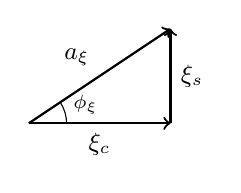
\begin{tikzpicture}[scale=1.2]
            \draw[thick, ->] (0,0) -- (1.5,0) node[midway, below] {\small $\xi_c$};
            \draw[thick, ->] (1.5,0) -- (1.5,1.0) node[midway, right] {\small $\xi_s$};
            \draw[thick, ->] (0,0) -- (1.5,1.0) node[midway, above left] {\small $a_\xi$};
            \draw (0.4,0) arc (0:33.69:0.4);
            \node at (0.6,0.2) {\scriptsize $\phi_\xi$};
        \end{tikzpicture}
    \end{minipage}

    \tcbline 
    
    \textbf{统计特性} (设 $\xi(t)$ 均值0,方差 $\sigma_{\xi}^2$):
    \begin{enumerate}
        \item $\xi_c(t), \xi_s(t)$ 均为高斯过程,均值0,方差 $\sigma_{\xi}^2$。
        \item \textbf{重要结论}:同一时刻,$\xi_c$ 与 $\xi_s$ \textbf{互不相关} (即统计独立)。
        \item \textbf{包络 $a_{\xi}$ (瑞利分布)}:$f(a_{\xi}) = \frac{a_{\xi}}{\sigma_{\xi}^2} e^{-\frac{a_{\xi}^2}{2\sigma_{\xi}^2}}, \ (a_{\xi} \geq 0)$
        \item \textbf{相位 $\phi_{\xi}$ (均匀分布)}:$f(\phi_{\xi}) = \frac{1}{2\pi}, \ (0 \leq \phi_{\xi} \leq 2\pi)$
    \end{enumerate}
\end{kbox}

\begin{kbox}{7. 白噪声与带限噪声}
    \textbf{基本概念}:
    \begin{itemize}
        \item \textbf{白噪声}:在整个频带内功率谱密度 (PSD) 都平坦的噪声。
        \item \textbf{高斯白噪声}:概率分布服从高斯分布,且 PSD 均匀的噪声。
        \item \textbf{带限白噪声}:白噪声通过有限带宽信道或滤波器后的噪声。
    \end{itemize}

    \tcbline

    \textbf{理想白噪声}:
    \begin{itemize}
        \item PSD (双边):$P_n(f) = n_0 / 2$
        \item 自相关:$R(\tau) = \frac{n_0}{2} \delta(\tau)$
    \end{itemize}
    
    \textbf{低通白噪声 (LPF, 截止 $f_H$)}:
    \[ R(\tau) = n_0 f_H \frac{\sin 2\pi f_H \tau}{2\pi f_H \tau} = n_0 f_H \operatorname{Sa}(2\pi f_H \tau) \] 
    
    \textbf{带通白噪声 (BPF, 带宽 $B$)}:
    \[ R(\tau) = n_0 B \frac{\sin \pi B \tau}{\pi B \tau} \cos 2\pi f_c \tau, \quad N = n_0 B \]
\end{kbox}

\begin{kbox}{8. 正弦波 + 窄带高斯噪声}
    \textbf{包络 $z$ 服从莱斯 (Rice) 分布}:
    \[ f(z) = \frac{z}{\sigma_n^2} \exp\left[-\frac{z^2 + A^2}{2\sigma_n^2}\right] I_0\left(\frac{Az}{\sigma_n^2}\right) \]
    ($A$: 信号振幅, $\sigma_n^2$: 噪声方差, $I_0$: 修正贝塞尔)
\end{kbox}       % 核心结论 & 矢量图
    \definecolor{mainblue}{RGB}{20, 80, 180}
\definecolor{fillblue}{RGB}{220, 230, 255}

\begin{examplebox}{补充:窄带过程推导与图解}
    \textbf{1. 正交分解推导细节}:
    利用三角公式展开 $\xi(t) = a_\xi(t) \cos[\omega_c t + \phi_\xi(t)]$:
    \begin{align*}
        \xi(t) &= a_\xi [\cos \phi_\xi \cos \omega_c t - \sin \phi_\xi \sin \omega_c t] \\
               &= \underbrace{[a_\xi \cos \phi_\xi]}_{\xi_c(t)} \cos \omega_c t - \underbrace{[a_\xi \sin \phi_\xi]}_{\xi_s(t)} \sin \omega_c t
    \end{align*}
    转换关系:
    \[ a_\xi = \sqrt{\xi_c^2 + \xi_s^2}, \quad \phi_\xi = \arctan(\xi_s / \xi_c) \]

    \tcbline

    \textbf{2. 概率密度函数图示}:
    \begin{center}
        \begin{tikzpicture}[font=\small]
            % --- 左图:瑞利分布 ---
            \begin{axis}[
                name=plot1,
                width=0.48\textwidth, height=5.5cm,
                axis lines=middle,
                xmin=0, xmax=4.2, ymin=0, ymax=0.75,
                xlabel={$a_\xi$}, ylabel={$f(a_\xi)$},
                ticks=none,
                axis line style={-latex, thick, black!80},
                xlabel style={right}, ylabel style={above},
                title={\textbf{瑞利分布 (包络)}},
                % --- 修改处:向上移动标题 15pt,并稍微加大字号 ---
                title style={yshift=15pt, font=\large}, 
                clip=false
            ]
                % 1. 绘制面积条带
                \fill[fillblue] (axis cs:1.2, 0) rectangle (axis cs:1.35, 0.48);
                
                % 2. 瑞利曲线
                \addplot[thick, mainblue, domain=0:4.0, samples=200] {x*exp(-x^2/2)};
                
                % 3. 均值虚线
                \draw[dashed, thick, black!60] (axis cs:1.253, 0) -- (axis cs:1.253, 0.455);
                
                % 4. 底部坐标标注
                \node[below] at (axis cs:1.253, 0) {$\sqrt{\frac{\pi}{2}}\sigma_\xi$};
                
                % 5. 文本公式
                \node[right, align=left] at (axis cs:1.8, 0.5) {
                    均值 $=\sqrt{\frac{\pi}{2}}\sigma_\xi$ \\[0.5em]
                    方差 $=\frac{4-\pi}{2}\sigma_\xi^2$
                };
                
                % 6. "等面积" 标注
                \node[coordinate, pin={[pin edge={black, thin}, align=center]120:等面积}] at (axis cs:1.27, 0.25) {};
                
            \end{axis}

            % --- 右图:均匀分布 ---
            \begin{axis}[
                at={(plot1.outer east)}, anchor=outer west,
                width=0.48\textwidth, height=5.5cm,
                axis lines=middle,
                xmin=0, xmax=7.5, ymin=0, ymax=0.35,
                xlabel={$\phi_\xi$}, ylabel={$f(\phi_\xi)$},
                ticks=none,
                axis line style={-latex, thick, black!80},
                xlabel style={right}, ylabel style={above},
                title={\textbf{均匀分布 (相位)}},
                % --- 修改处:同样向上移动标题 15pt ---
                title style={yshift=15pt, font=\large},
                clip=false
            ]
                % 1. 均匀分布矩形
                \draw[thick, mainblue, fill=fillblue!30] (axis cs:0, 0) -- (axis cs:0, 0.2) -- (axis cs:6.283, 0.2) -- (axis cs:6.283, 0);
                
                % 2. 坐标标注
                \node[below left] at (axis cs:0,0) {$0$};
                \node[below] at (axis cs:6.283,0) {$2\pi$};
                \node[left] at (axis cs:0, 0.2) {$\frac{1}{2\pi}$};
                
                % 3. 装饰虚线
                \draw[dashed, black!40] (axis cs:6.283, 0) -- (axis cs:6.283, 0.2);
                
            \end{axis}
        \end{tikzpicture}
    \end{center}
\end{examplebox} % 详细推导 & 分布图解
    
    \begin{kbox}{9. 随机过程维度的物理意义(补充)}
    \textbf{为什么会有“一维”和“二维”之分?}
    \begin{itemize}
        \item \textbf{一维 PDF ($f_1$) —— 看“切片”(静态)}:
        固定某一时刻 $t$ 观察。它决定了信号的\textbf{均值}和\textbf{方差}(即平均功率、直流/交流分量)。
        \item \textbf{二维 PDF ($f_2$) —— 看“关联”(动态)}:
        固定两个时刻 $t_1, t_2$ 观察。它包含了\textbf{相关性}信息。不看二维就无法定义自相关函数 $R(\tau)$,也就无法得到功率谱密度 (PSD)。
    \end{itemize}
    
    \tcbline
    
    \textbf{为什么通信中主要关注 1维 和 2维?}
    虽然理论上随机过程有无限维 ($n$维),但在工程应用中:
    \begin{enumerate}
        \item \textbf{高斯过程的特性}:由其 1维(均值)和 2维(自相关/协方差)特性\textbf{完全决定}。即知道了前两维,就确定了整个随机过程。
        \item \textbf{广义平稳 (WSS)}:工程主要处理 WSS 过程,其定义标准仅依赖于均值(1维特性)和自相关函数(2维特性)。
    \end{enumerate}
\end{kbox}

\begin{examplebox}{例 3.2(1):求自相关函数 (详细推导版)}
    \textbf{题目描述}:已知随机过程 $\xi(t)$ 的功率谱密度 $P_\xi(f)$ 如图所示(三角形波 + 直流冲激),求自相关函数 $R(\tau)$。
        \begin{center}
            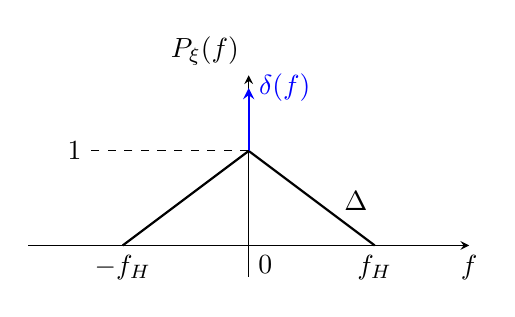
\begin{tikzpicture}[>=stealth, scale=0.8]
                % --- 坐标轴调整 ---
                \draw[->] (-3.5,0) -- (3.5,0) node[below] {$f$};
                % [修改点1]: 将纵轴标签移到左上方,避免与右侧的 delta(f) 标签打架
                \draw[->] (0,-0.5) -- (0,2.7) node[above left] {$P_{\xi}(f)$};
                % --- 三角波 ---
                \draw[thick] (-2,0) -- (0,1.5) -- (2,0);
                % [修改点2]: 将三角符号向右移动 (x坐标从 1.2 改为 1.7)
                \node at (1.7, 0.7) {$\Delta$};
                % --- 直流冲击 delta(f) ---
                % 保持粗线条和蓝色,绘制在坐标轴上方,标签在右侧
                \draw[->, thick, blue] (0,1.5) -- (0,2.5) node[right] {$\delta(f)$};
                % --- 刻度 ---
                \node[below] at (-2,0) {$-f_H$};
                \node[below] at (2,0) {$f_H$};
                \node[below right] at (0,0) {$0$};
                
                % --- 标注峰值 ---
                \draw[dashed] (0,1.5) -- (-2.5, 1.5);
                \node[left] at (-2.5, 1.5) {$1$};
            \end{tikzpicture}
        \end{center}
    
    \tcbline
    
    \textbf{1. 预备知识:傅里叶变换对的推导}
    
    为了求解本题,我们需要建立门函数 $g_{f_H}(f)$ 与抽样函数 $Sa(\cdot)$ 的对应关系。这里提供两种推导方法:
    
    \textbf{方法一:定义法 (积分推导)}
    \begin{itemize}
        \item \textbf{变量对照表}:
        \begin{center}
            \renewcommand{\arraystretch}{1.2}
            \begin{tabular}{|c|c|}
                \hline
                $\omega$ & $2\pi f$ \\
                \hline
                $f$ & $\frac{\omega}{2\pi}$ \\
                \hline
            \end{tabular}
        \end{center}
        \item \textbf{推导}:
        \[
        \begin{aligned}
            \mathcal{F}^{-1}[g_{f_H}(f)] &= \int_{-f_H/2}^{f_H/2} 1 \cdot e^{j2\pi f \tau} df \\
            &= \left[ \frac{e^{j2\pi f \tau}}{j2\pi \tau} \right]_{-f_H/2}^{f_H/2} \\
            &= \frac{e^{j\pi f_H \tau} - e^{-j\pi f_H \tau}}{j2\pi \tau} \\
            &= \frac{\sin(\pi f_H \tau)}{\pi \tau} = f_H Sa(\pi f_H \tau)
        \end{aligned}
        \]
    \end{itemize}

    \textbf{方法二:利用线性性质与尺度变换 (根据手写笔记)}
    \begin{itemize}
        \item \textbf{Step 1: 标准变换对} (门宽为 1)
        \[ g_1(f) \leftrightarrow Sa(\pi \tau) \]
        \item \textbf{Step 2: 频域尺度变换} (引入 $f_H$)
        利用性质 $X(f/k) \leftrightarrow |k|x(k\tau)$。令 $k=f_H$:
        \[ g_{f_H}(f) = g_1\left(\frac{f}{f_H}\right) \leftrightarrow f_H Sa(\pi f_H \tau) \]
        \item \textbf{Step 3: 线性性质/幅度缩放} (构造题目系数)
        题目需构造系数 $A = \frac{1}{\sqrt{f_H}}$。求 $\frac{1}{\sqrt{f_H}} g_{f_H}(f)$ 的逆变换。
        两边同乘 $\frac{1}{\sqrt{f_H}}$:
        \[ \frac{1}{\sqrt{f_H}} g_{f_H}(f) \leftrightarrow \frac{1}{\sqrt{f_H}} \cdot [f_H Sa(\pi f_H \tau)] \]
        化简右边系数 $\frac{f_H}{\sqrt{f_H}} = \sqrt{f_H}$,得最终变换对:
        \[ \boxed{\frac{1}{\sqrt{f_H}} g_{f_H}(f) \leftrightarrow \sqrt{f_H} Sa(\pi f_H \tau)} \]
    \end{itemize}

    \tcbline
    
    \textbf{2. 功率谱密度 $P_\xi(f)$ 的分解与参数求解}
    
    由图可知,$P_\xi(f) = \Delta(f) + \delta(f)$。
    
    \textbf{求解三角形 $\Delta(f)$ 的构成:}
    三角形可视为两个相同门函数 $A \cdot g_{f_H}(f)$ 的卷积。
    \[ \Delta(f) = [A \cdot g_{f_H}(f)] * [A \cdot g_{f_H}(f)] \]
    
    根据卷积几何性质:
    \begin{itemize}
        \item 卷积后高度 = $A^2 \cdot \text{门宽} = A^2 f_H$
    \end{itemize}
    
    由图知三角形顶点高度为 $1$,故 $A^2 f_H = 1 \implies A = \frac{1}{\sqrt{f_H}}$。
    即:
    \[ \Delta(f) = \left[ \frac{1}{\sqrt{f_H}} g_{f_H}(f) \right] * \left[ \frac{1}{\sqrt{f_H}} g_{f_H}(f) \right] \]

    \tcbline
    
    \textbf{3. 求解自相关函数 $R(\tau)$}
    
    利用维纳-辛钦定理及“频域卷积 $\leftrightarrow$ 时域相乘”:
    
    \[
    \begin{aligned}
        R(\tau) &= \mathcal{F}^{-1}[\Delta(f)] + \mathcal{F}^{-1}[\delta(f)] \\
        &= \mathcal{F}^{-1}\left\{ \left[ \frac{1}{\sqrt{f_H}} g_{f_H}(f) \right] * \left[ \frac{1}{\sqrt{f_H}} g_{f_H}(f) \right] \right\} + 1 \\
        &= \left( \mathcal{F}^{-1}\left[ \frac{1}{\sqrt{f_H}} g_{f_H}(f) \right] \right)^2 + 1 
    \end{aligned}
    \]
    代入步骤1中推导出的结论:
    \[
    \begin{aligned}
        R(\tau) &= \left( \sqrt{f_H} Sa(\pi f_H \tau) \right)^2 + 1 \\
        &= f_H Sa^2(\pi f_H \tau) + 1
    \end{aligned}
    \]
    
    \tcbline
    \textbf{4. 功率计算}
    \begin{itemize}
        \item 平均功率 $R(0) = f_H + 1$
        \item 直流功率 $R(\infty) = 1$
        \item 交流功率 $\sigma^2 = f_H$
    \end{itemize}
\end{examplebox}

\clearpage  % 用于强制换页

% chapter/chapter03.tex

\section{信道}

\begin{kbox}{1. 信道模型}
    \textbf{调制信道 (Modulation Channel)}:
    \begin{itemize}
        \item 入出关系:
        \[ r(t) = k(t) \cdot s_i(t) + n(t) \]
        \item $k(t)$:乘性干扰 (反映信道时变特性)
        \item $n(t)$:加性噪声
    \end{itemize}
    
    \tcbline
    
    \textbf{编码信道 (Encoding Channel)} (二进制):
    \begin{itemize}
        \item 正确传输概率:$P(0/0) + P(1/0) = 1$
        \item \textbf{误码率}:
        \[ P_e = P(0)P(1/0) + P(1)P(0/1) \]
    \end{itemize}
\end{kbox}

\begin{kbox}{2. 恒参信道特性}
    \textbf{传输函数}:$H(\omega) = |H(\omega)| e^{j\varphi(\omega)}$
    
    \textbf{无失真传输条件}:
    \begin{enumerate}
        \item \textbf{幅频特性}:$|H(\omega)| = K$ (常数)
        \item \textbf{相频特性}:$\varphi(\omega) = \omega t_d$ (通过原点的直线)
        \item \textbf{群迟延}:$\tau(\omega) = \frac{d\varphi(\omega)}{d\omega} = t_d$ (常数)
    \end{enumerate}
    
    \textbf{时域响应}:
    \[ h(t) = K\delta(t - t_d) \Longrightarrow s_o(t) = K s(t - t_d) \]
\end{kbox}

\begin{kbox}{3. 随参信道与多径效应}
    \textbf{接收信号模型} ($n$ 条路径):
    \[ r(t) = \sum_{i=1}^n a_i(t) \cos \omega_c [t - \tau_i(t)] = V(t) \cos[\omega_c t + \varphi(t)] \]
    多径效应导致信号包络 $V(t)$ 和相位 $\varphi(t)$ 随机起伏。
    
    \tcbline
    
    \textbf{频率选择性衰落}:
    \begin{itemize}
        \item \textbf{相关带宽}:$\Delta f = 1/\tau_m$ ($\tau_m$ 为最大多径时延差)
        \item \textbf{工程经验公式} (避免频选衰落):
        \begin{itemize}
            \item 信号带宽:$B_s \leq (1/3 \sim 1/5) \Delta f$
            \item 码元宽度:$T_s \geq (3 \sim 5) \tau_m$
        \end{itemize}
    \end{itemize}
\end{kbox}

\begin{kbox}{4. 信道噪声 (高斯白噪声)}
    \textbf{统计特性}:
    \begin{itemize}
        \item 双边 PSD:$P_n(f) = n_0 / 2$ (W/Hz)
        \item 自相关:$R_n(\tau) = \frac{n_0}{2} \delta(\tau)$
        \item 一维 PDF (正态分布):
        \[ f_n(v) = \frac{1}{\sqrt{2\pi}\sigma_n} \exp\left(-\frac{v^2}{2\sigma_n^2}\right) \]
    \end{itemize}
    
    \textbf{功率计算}:
    \begin{itemize}
        \item 噪声功率:$N = \int_{-\infty}^{\infty} P_n(f) df$
        \item 等效带宽:$B_n = \frac{\int_0^{\infty} P_n(f) df}{P_n(f_0)}$
    \end{itemize}
\end{kbox}

\begin{kbox}{5. 信道容量 (Channel Capacity)}
    \textbf{离散信道}:
    \[ C = \max_{P(x)} [H(x) - H(x/y)] \quad (\text{b/符号}) \]
    其中 $H(x/y)$ 为损失信息量(平均条件熵)。
    
    \tcbline
    
    \textbf{连续信道 (香农公式 Shannon Formula)}:
    \[ C = B \log_2 \left( 1 + \frac{S}{N} \right) = B \log_2 \left( 1 + \frac{S}{n_0 B} \right) \]
    \begin{itemize}
        \item $B$:带宽 (Hz),$S$:信号功率 (W)
        \item $n_0$:噪声单边 PSD (W/Hz)
    \end{itemize}
    
    \textbf{带宽无限大极限}:
    \[ \lim_{B \to \infty} C \approx 1.44 \frac{S}{n_0} \]
    这意味着信道容量有极限值,不能通过无限增加带宽来无限增加容量。
\end{kbox}

\clearpage  % 用于强制换页

\section{信源编码}

\begin{kbox}{抽样定理 (Sampling Theorem)}
    \begin{itemize}
        \item \textbf{低通模拟信号抽样定理} \pptpage{12}
        \begin{itemize}
            \item \textbf{条件}:为了无失真恢复原信号,抽样速率 $f_s$ 需满足:
            \begin{equation}
                f_s \ge 2f_H \quad \text{且} \quad T_s \le \frac{1}{2f_H}
            \end{equation}
            其中 $f_H$ 为信号最高频率。
            \item \textbf{奈奎斯特速率}:$f_s = 2f_H$
            \item \textbf{奈奎斯特间隔}:$T_s = \frac{1}{2f_H}$
        \end{itemize}
        
        \item \textbf{理想抽样 (Ideal Sampling)} \pptpage{13}
        \begin{itemize}
            \item \textbf{时域}:利用单位冲激序列 $\delta_T(t)$ 进行乘积:
            % --- 修正:使用 split 环境将长公式换行对齐 ---
            \begin{equation}
            \begin{split}
                m_s(t) &= m(t)\sum_{n=-\infty}^{\infty}\delta(t-nT_s) \\
                       &= \sum_{n=-\infty}^{\infty}m(nT_s)\delta(t-nT_s)
            \end{split}
            \end{equation}
            \item \textbf{频域}:频谱以 $f_s$ 为周期搬移:
            \begin{equation}
                M_s(f) = \frac{1}{T_s}\sum_{n=-\infty}^{\infty}M(f-nf_s)
            \end{equation}
        \end{itemize}

        \item \textbf{平顶抽样与孔径失真} \pptpage{26}
        \begin{itemize}
            \item \textbf{产生}:理想抽样脉冲经过形状为 $h(t)$ 的保持电路。
            \item \textbf{频域关系}:
            \begin{equation}
                M_H(f) = M_s(f) \cdot H(f)
            \end{equation}
            \item \textbf{孔径失真}:由 $H(f) = T_s \text{Sa}(\pi f T_s)$ (矩形脉冲) 引起的高频衰减,需在接收端使用 \textbf{修正滤波器} 进行补偿。
        \end{itemize}
    \end{itemize}
\end{kbox}

\begin{kbox}{量化 (Quantization)}
    \begin{itemize}
        \item \textbf{均匀量化 (Uniform Quantization)} \pptpage{32}
        \begin{itemize}
            \item \textbf{量化间隔}:$\Delta v = \frac{b-a}{M}$
            \item \textbf{量化噪声功率} (重要结论):
            \begin{equation}
                N_q = \frac{(\Delta v)^2}{12}
            \end{equation}
            \item \textbf{信号量噪比 ($S/N_q$)} \pptpage{34}:
            % 使用 multline 确保长公式能够适应窄栏
            \begin{multline}
                (S/N_q)_{\text{dB}} \approx \\ 4.8 + 6n + 10\lg(S/x_{max}^2)
            \end{multline}
            \textbf{结论}:编码位数 $n$ 每增加 1 bit,信噪比提高约 \textbf{6dB}。
        \end{itemize}

        \item \textbf{非均匀量化 (Non-uniform)} \pptpage{38}
        \begin{itemize}
            \item \textbf{原理}:先压缩 (Compress),再均匀量化,最后扩张 (Expand)。目的:提高\textbf{小信号}的量噪比。
            \item \textbf{A律压缩特性} (A-Law, 欧/中标准, $A=87.6$) \pptpage{44}:
            % 微调格式,确保分数在窄栏中不溢出
            \begin{equation}
                y = \begin{cases} 
                \frac{Ax}{1+\ln A}, & 0 < x \le \frac{1}{A} \\[6pt] % 增加行间距
                \frac{1+\ln(Ax)}{1+\ln A}, & \frac{1}{A} \le x \le 1 
                \end{cases}
            \end{equation}
            \item \textbf{$\mu$律压缩特性} (美/日标准, $\mu=255$):
            \begin{equation}
                y = \frac{\ln(1+\mu x)}{\ln(1+\mu)}, \quad 0 \le x \le 1
            \end{equation}
            \item \textbf{改善度}:$[Q]_{\text{dB}} = 20\lg y'$,即取决于压缩曲线斜率。
        \end{itemize}
    \end{itemize}
\end{kbox}

\begin{kbox}{脉冲编码调制 (PCM)}
    \begin{itemize}
        \item \textbf{基本参数} \pptpage{72}
        设模拟信号最高频率为 $f_H$,抽样率为 $f_s$,编码位数为 $N$。
        \item \textbf{信息传输速率 (比特率)}:
        \begin{equation}
            R_b = f_s \cdot N \ge 2f_H \cdot N
        \end{equation}
        \item \textbf{传输带宽} (第一零点带宽):
        \begin{equation}
            B = R_b = f_s \cdot N \quad (\text{NRZ矩形})
        \end{equation}
        \item \textbf{典型应用:数字电话}
        \begin{itemize}
            \item 话音带宽 $B \approx 3.4\text{kHz} \to f_s = 8000\text{Hz}$
            \item 量化位数 $N=8$ (A律13折线)
            \item \textbf{比特率}:$R_b = 8000 \times 8 = \mathbf{64\text{kbps}}$
        \end{itemize}
    \end{itemize}
\end{kbox}

\clearpage  % 用于强制换页

\section{数字基带传输}

\subsection{数字基带信号的表示与编码}

\begin{kbox}{基带信号一般表达式 (随机脉冲序列) \pptpage{15}}
    \begin{equation*}
        s(t) = \sum_{n=-\infty}^{\infty} a_n g(t - nT_B)
    \end{equation*}
    \begin{itemize}
        \item $a_n$:第 $n$ 个码元的电平取值(统计独立的随机量)
        \item $g(t)$:单个脉冲波形;$T_B$:码元持续时间
    \end{itemize}
\end{kbox}

% 【修改点1】添加垂直间距,解决挨得太近的问题
\vspace{1em} 

\begin{enumerate}
    \item \textbf{差分编码与译码(相对码)} \pptpage{13}
    \begin{itemize}
        \item \textbf{编码}:$b_n = a_n \oplus b_{n-1}$ (克服相位模糊)
        \item \textbf{译码}:$a_n = b_n \oplus b_{n-1}$
    \end{itemize}
    
    \item \textbf{多电平(四电平)定义} \pptpage{14}
    \begin{itemize}
        \item 映射关系:$00 \to +3E,\; 01 \to +E,\; 10 \to -E,\; 11 \to -3E$
    \end{itemize}
\end{enumerate}

\subsection{基带信号的功率谱密度 (PSD)}

\begin{kbox}{功率谱分解通用公式 \pptpage{17-18}}
    \begin{equation*}
        P_s(f) = P_u(f) + P_v(f)
    \end{equation*}
    \tcblower
    \begin{itemize}
        \item \textbf{连续谱(交变波)}:
        \[ P_u(f) = f_B p(1-p) \left| G_1(f) - G_2(f) \right|^2 \]
        
        \item \textbf{离散谱(稳态波)}:
        % 【修改点2】使用 aligned 环境换行,防止公式超出分栏宽度
        \[
        \begin{aligned}
            P_v(f) = & \sum_{m=-\infty}^{\infty} \Big| f_B [  p G_1(mf_B) \\
            & + (1-p)G_2(mf_B)] \Big|^2 \delta(f - mf_B)
        \end{aligned}
        \]
        
        \item \textbf{离散谱消失条件}:$p = \frac{1}{1 - g_1(t)/g_2(t)}$
    \end{itemize}
\end{kbox}

\noindent\textbf{典型波形的功率谱密度:}
\begin{itemize}
    \item \textbf{单极性 NRZ} \pptpage{19}:
    $P_s(f) = \frac{1}{4} T_s \mathrm{Sa}^2(\pi f T_s) + \frac{1}{4} \delta(f)$
    
    \item \textbf{单极性 RZ (占空比1/2)} \pptpage{20}:
    $P_s(f) = \frac{1}{16} T_s \mathrm{Sa}^2(\frac{\pi f T_s}{2}) + \frac{1}{16} \sum_{m} \mathrm{Sa}^2(\frac{m\pi}{2}) \delta(f - mf_s)$
    
    \item \textbf{双极性等概 NRZ ($p=1/2$)} \pptpage{21}:
    $P_s(f) = T_s \mathrm{Sa}^2(\pi f T_s)$ (\textcolor{alertred}{无离散谱、无直流})
\end{itemize}

\subsection{码间干扰 (ISI) 与奈奎斯特准则}

\begin{kbox}{接收抽样点信号分解 \pptpage{41-43}}
    % 【修改点3】分三行对齐,解决长公式和下括号导致的溢出
    \[
    \begin{aligned}
        r(kT_s + t_0) = & \underbrace{a_k h(t_0)}_{\text{有用信号}} \\
        & + \underbrace{\sum_{n \neq k} a_n h(kT_s + t_0 - nT_s)}_{\text{码间干扰 ISI}} \\
        & + \underbrace{n_R(kT_s + t_0)}_{\text{噪声}}
    \end{aligned}
    \]
    其中 $h(t) = \mathcal{F}^{-1}\{G_T(\omega)C(\omega)G_R(\omega)\}$ 为系统总响应。
\end{kbox}

\subsubsection*{1. 奈奎斯特第一准则 (无ISI准则)}
\begin{itemize}
    \item \textbf{时域条件} \pptpage{50}:
    \[ h(mT_s) = \begin{cases} 1, & m=0 \\ 0, & m \neq 0 \end{cases} \]
    \item \textbf{频域条件} \pptpage{52, 55}:
    \[ \sum_{i=-\infty}^{\infty} H\left(\omega + \frac{2\pi i}{T_s}\right) = T_s, \quad |\omega| \leq \frac{\pi}{T_s} \]
\end{itemize}

\subsubsection*{2. 系统带宽指标}
\begin{enumerate}
    \item \textbf{理想低通系统} \pptpage{58-59}:
    \begin{itemize}
        \item 奈奎斯特带宽:$B = \frac{1}{2T_B} = f_N$
        \item 最高频带利用率:$\eta = R_B/B = 2$ (Baud/Hz)
    \end{itemize}
    \item \textbf{余弦滚降系统} \pptpage{61-62}:
    \begin{itemize}
        \item 带宽:$B = (1+\alpha)f_N$ ($\alpha$ 为滚降系数)
        \item 利用率:$\eta = \frac{2}{1+\alpha}$ (Baud/Hz)
    \end{itemize}
\end{enumerate}

\subsection{基带系统的抗噪声性能}

\begin{itemize}
    \item \textbf{噪声方差} \pptpage{73}:$\sigma_n^2 = \int_{-\infty}^{\infty} \frac{n_0}{2} |G_R(f)|^2 df$
    \item \textbf{误码率 $P_e$ 与最佳门限 $V_d^*$}:
\end{itemize}

\begin{kbox}{误码率公式速查}
    \textbf{1. 双极性基带系统} \pptpage{78-79}
    \begin{itemize}
        \item 最佳门限:$V_d^* = \frac{\sigma_n^2}{2A} \ln \frac{P(0)}{P(1)}$
        \item \textbf{等概时 ($P(0)=P(1)$)}:
        \[ V_d^* = 0, \quad P_e = \frac{1}{2} \operatorname{erfc}\left(\frac{A}{\sqrt{2}\sigma_n}\right) \]
    \end{itemize}
    
    \tcblower
    
    \textbf{2. 单极性基带系统} \pptpage{81-82}
    \begin{itemize}
        \item 最佳门限:$V_d^* = \frac{A}{2} + \frac{\sigma_n^2}{A} \ln \frac{P(0)}{P(1)}$
        \item \textbf{等概时}:
        \[ V_d^* = \frac{A}{2}, \quad P_e = \frac{1}{2} \operatorname{erfc}\left(\frac{A}{2\sqrt{2}\sigma_n}\right) \]
    \end{itemize}
\end{kbox}

\subsection{部分响应系统与时域均衡}

\subsubsection*{1. 第I类部分响应 (奈奎斯特第二准则)}
\begin{itemize}
    \item \textbf{编码}:$c_k = a_k + a_{k-1}$
    \item \textbf{频域} \pptpage{87}:$G(f) = 2T_s \cos(\pi f T_s), \quad |f| \leq \frac{1}{2T_s}$
    \item \textbf{预编码} \pptpage{90}:$b_k = a_k \oplus b_{k-1}$ (防止差错传播)
\end{itemize}

\subsubsection*{2. 时域均衡 (TDE)}
\begin{itemize}
    \item \textbf{横向滤波器输出} \pptpage{98}:$y_k = \sum_{n=-N}^{N} C_n x_{k-n}$
    \item \textbf{设计目标}:使 $y_k$ 满足无 ISI 条件。
    \item \textbf{均衡器频率响应} \pptpage{96}:
    \[ T(\omega) = \frac{T_B}{\sum_i H(\omega + \frac{2\pi i}{T_B})} \]
\end{itemize}

\subsection{实验评估:眼图 \pptpage{103}}
\begin{itemize}
    \item \textbf{眼睛张开度}:反映 ISI 和噪声强弱(开口大则ISI小)。
    \item \textbf{最佳抽样时刻}:眼睛张开最大的时刻。
    \item \textbf{斜边斜率}:反映对定时误差的灵敏度(斜率越大越敏感)。
\end{itemize}

\clearpage  % 用于强制换页

\section{数字带通传输系统}

% --- 第一部分:基础模型 ---
\begin{kbox}{信号基础模型与通用定义}
    \begin{itemize}
        \item \textbf{已调信号通用形式} \pptpage{14, 16}
        $$ u_M(t) = u_c(t) \cos[\omega_c t + \varphi_c(t)] $$
        \item \textbf{正交表示法} \pptpage{122, 124}
        $$ s(t) = I(t) \cos \omega_c t - Q(t) \sin \omega_c t $$
        \item \textbf{关键参数定义}
        \begin{itemize}
            \item \textbf{信噪比 (SNR)}: $r = \frac{a^2}{2\sigma_n^2}$ ($a$: 幅度, $\sigma_n^2$: 噪声功率) \pptpage{55}
            \item \textbf{速率关系}: $R_b = R_B \log_2 M$ \pptpage{100}
            \item \textbf{频带利用率} $\eta$ (bps/Hz): \pptpage{147}
            $$ \eta = \frac{R_b}{B} = \frac{\log_2 M}{1+\alpha} \quad (\alpha: \text{滚降系数}) $$
        \end{itemize}
    \end{itemize}
\end{kbox}

% --- 第二部分:二进制调制 (ASK/FSK) ---
\begin{kbox}{二进制调制 (2ASK / 2FSK)}
    \begin{enumerate}
        \item \textbf{2ASK (OOK)}
        \begin{itemize}
            \item 时域: $e_{2ASK}(t) = s(t) \cos \omega_c t$ \pptpage{18}
            \item \textbf{功率谱密度 (PSD)}: \pptpage{38}
            $$ P_{2ASK}(f) = \frac{1}{4} [P_s(f+f_c) + P_s(f-f_c)] $$
            \item 带宽: $\bm{B_{2ASK} = 2R_B}$ \pptpage{39}
            \item 误码率 $P_e$:
            \begin{itemize}
                \item 相干: $\frac{1}{2} \text{erfc}(\sqrt{r/4})$ \pptpage{54}
                \item 包络 (大信噪比): $\approx \frac{1}{2} e^{-r/4}$ \pptpage{62}
            \end{itemize}
        \end{itemize}
        
        \item \textbf{2FSK}
        \begin{itemize}
            \item 时域: $s_1(t) \cos \omega_1 t + s_2(t) \cos \omega_2 t$ \pptpage{23}
            \item 带宽: $\bm{B_{2FSK} \approx |f_2 - f_1| + 2R_B}$ \pptpage{42}
            \item 误码率 $P_e$:
            \begin{itemize}
                \item 相干: $\frac{1}{2} \text{erfc}(\sqrt{r/2})$ \pptpage{69}
                \item 非相干: $\frac{1}{2} e^{-r/2}$ \pptpage{74}
            \end{itemize}
        \end{itemize}
    \end{enumerate}
\end{kbox}

% --- 第三部分:二进制调制 (PSK) ---
\begin{kbox}{二进制相位调制 (2PSK / 2DPSK)}
    \begin{enumerate}
        \item \textbf{2PSK (BPSK)}
        \begin{itemize}
            \item 时域: $e_{2PSK}(t) = s(t) \cos \omega_c t$ ($a_n \in \{+1, -1\}$) \pptpage{29}
            \item 带宽: $B_{2PSK} = 2R_B$ \pptpage{40}
            \item \textcolor{alertred}{\textbf{误码率 (相干)}}: $\bm{P_e = \frac{1}{2} \text{erfc}(\sqrt{r})}$ \pptpage{83}
            \item \textit{注:2PSK在二进制中抗噪声性能最优。}
        \end{itemize}
        
        \item \textbf{2DPSK}
        \begin{itemize}
            \item \textbf{差分编码}: $b_n = a_n \oplus b_{n-1}$ \pptpage{33}
            \item 误码率 $P_e$:
            \begin{itemize}
                \item 相干+码反变换: $\approx \frac{1}{\sqrt{\pi r}} e^{-r}$ (存在误码扩散) \pptpage{87}
                \item 差分相干: $\frac{1}{2} e^{-r}$ \pptpage{91}
            \end{itemize}
        \end{itemize}
    \end{enumerate}
\end{kbox}

% --- 第四部分:抗噪声性能大总结 (新增表格) ---
\begin{kbox}{二进制误码率近似公式对比表 (大信噪比) \pptpage{91-95}}
    \centering
    \renewcommand{\arraystretch}{1.5}
    \begin{tabular}{|c|c|c|}
        \hline
        \textbf{调制方式} & \textbf{相干解调 (近似)} & \textbf{非相干/差分 (近似)} \\
        \hline
        \textbf{2ASK} & $\frac{1}{\sqrt{\pi r}}e^{-r/4}$ & $\frac{1}{2}e^{-r/4}$ \\
        \hline
        \textbf{2FSK} & $\frac{1}{\sqrt{\pi r}}e^{-r/2}$ & $\frac{1}{2}e^{-r/2}$ \\
        \hline
        \textbf{2PSK} & $\frac{1}{\sqrt{\pi r}}e^{-r}$ & — \\
        \hline
        \textbf{2DPSK} & $\frac{1}{\sqrt{\pi r}}e^{-r}$ & $\frac{1}{2}e^{-r}$ \\
        \hline
    \end{tabular}
    \vspace{0.5em}
    \begin{itemize}
        \item \textbf{信噪比关系 (同误码率)}: 
        $$ r_{2ASK} = 2r_{2FSK} = 4r_{2PSK} \quad (\text{分贝差 } 3dB, 6dB) $$
    \end{itemize}
\end{kbox}

% --- 第五部分:多进制调制 ---
\begin{kbox}{多进制调制系统 (M-ary)}
    \begin{enumerate}
        \item \textbf{MASK}: 
        \begin{itemize}
            \item 带宽: $B = \frac{2R_b}{\log_2 M}$ \pptpage{104}
            \item 误码率: $P_e = (1 - \frac{1}{M}) \text{erfc}(\sqrt{\frac{3}{M^2-1} r})$ \pptpage{156}
        \end{itemize}
        
        \item \textbf{MFSK}:
        \begin{itemize}
            \item 带宽: $B \approx |f_M - f_1| + 2R_B$ \pptpage{107}
            \item 非相干误码率: $P_e \approx \frac{M-1}{2} e^{-r/2}$ \pptpage{157}
        \end{itemize}

        \item \textbf{MPSK}:
        \begin{itemize}
            \item QPSK带宽: $B = R_b$ (频带利用率高) \pptpage{125}
            \item 误码率: $P_e \approx \text{erfc}(\sqrt{r} \sin \frac{\pi}{M})$ \pptpage{159}
        \end{itemize}
        
        \item \textbf{MQAM (重点)}:
        \begin{itemize}
            \item 时域: $e(t) = I(t) \cos \omega_c t - Q(t) \sin \omega_c t$ \pptpage{141}
            \item 带宽 (含滚降 $\alpha$): $\bm{B = \frac{(1+\alpha)R_b}{\log_2 M}}$ \pptpage{147}
        \end{itemize}
    \end{enumerate}
\end{kbox}

% --- 第六部分:性能总结 ---
\begin{kbox}{全章结论与演变规律 \pptpage{93, 161}}
    \begin{enumerate}
        \item \textbf{系统演变规律 (当 M 增大时)}
        \begin{itemize}
            \item \textbf{MASK / MPSK / MQAM}:
            \newline $\eta \uparrow$ (有效性变好), $P_e$ 性能 $\downarrow$ (可靠性变差)
            \item \textbf{MFSK}:
            \newline $\eta \downarrow$ (有效性变差), \textcolor{mainblue}{\textbf{$P_e$ 性能 $\uparrow$}} (可靠性变好,特例)
        \end{itemize}
        
        \item \textbf{核心一句话结论}:
        \begin{quote}
            \small
            \textit{“2PSK抗噪最好;2FSK最费带宽但简单;MQAM是现代通信在带宽受限信道中兼顾效率与性能的主流。”}
        \end{quote}
    \end{enumerate}
\end{kbox}

\end{document}